\documentclass[11pt,a4paper]{article}
\usepackage[utf8]{inputenc}
\usepackage[portuguese]{babel}
\usepackage[T1]{fontenc}
\usepackage[left=1.7cm,right=1.5cm,top=2.5cm,bottom=2cm]{geometry}
\usepackage{xcolor}
\definecolor{orange}{RGB}{255,127,0}
%\usepackage[dvipsnames]{xcolor}
\usepackage{titlesec}
\usepackage[utf8]{inputenc}
\usepackage[portuguese]{babel}
\usepackage[T1]{fontenc}
\usepackage{amsmath}
\usepackage{amsthm}
\usepackage{amsfonts}
\usepackage{amssymb}
\usepackage{graphicx}
\usepackage{stackengine}
\usepackage{accents}
\usepackage{xcolor}
\usepackage{bbm}
\usepackage{enumitem}
\usepackage{mathtools}
\usepackage{ mathrsfs }
\newtheorem{teo}{\underline{Teorema}}
\newtheorem*{defi}{\underline{Definição}}
\newtheorem{prop}{\underline{Proposição}}
\newtheorem{prop2}{\underline{Propriedade}}
\newtheorem*{col}{\underline{Corolário}}
\newtheorem{lema}{\underline{Lema}}
\usepackage{bbm}
\newcommand{\e}{\mathbb{E}}
\newcommand{\var}{\mathrm{Var}}
\newcommand{\cov}{\mathrm{Cov}}
\newcommand{\p}{\mathbb{P}}
\newcommand{\dis}{\displaystyle}
\usepackage{subfigure}
\title{Perfil de Consumo de Usuário de Jogos Eletrónicos}
\author{Carolina Martins, Daniel dos Santos, Fernanda Fernandes, Gabriel Mizuno, Isabelly  Almeida}
\usepackage{tasks}
\usepackage{exsheets}
\SetupExSheets[question]{type=exam}
\usepackage{makecell}
\usepackage{color, colortbl}
\date{ }
\usepackage{indentfirst}
\usepackage{float}
\usepackage{hyperref}
\hypersetup{colorlinks=true,linkcolor=red,citecolor=blue}
 
\begin{document}
 
\maketitle
 
\tableofcontents

\newpage
\section{Introdução}

Com o rápido e surpreendente crescimento da indústria dos jogos eletrónicos, como foi observado em 2016, onde a final do mundial do jogo League of Legends (LoL) teve mais telespectadores do que os sete (7) jogos da final da NBA (\href{https://bit.ly/2Dvdtw9}{\textcolor{blue}{LoL vs NBA}}) e em uma outra situação, onde lançamento dos principais jogos tiveram lucros maiores do que blockbusters feitos em Hollywood  (\href{https://bit.ly/2FfWHTk}{\textcolor{blue}{Filmes vs Jogos}}), a análise do perfil de consumo dos usuários torna-se cada vez mais necessária para conquista e fidelização de seus usurários. Essa pesquisa visa fazer essa analise, de maneira não muito profunda, sobre usuários que vivem no Brasil. 
\\ 
\\
 
\section{Metodologia}

Para a obtenção dos dados foi criado um formulário usando o Google Forms  e durante o período de 1 de Novembro de 2018 até 13 de Novembro de 2018 foi distribuído em grupo de discussão na plataforma do Facebook. Para a construção do formulário foi usado os seguintes critério:

\begin{enumerate}[label=(\roman*)]
\item Ser jogador independente da plataforma;
\item Ser brasileiro ou morar no Brasil.
\end{enumerate}

Depois de coletados os dados foram utilizados os software estatístico Rstudio e Excel, também foi necessário tratar a base de dados, pois durante a obtenção desses dados alguns voluntários colocaram respostas que não condiziam com a realidade do ser humano, sendo assim foram usados os seguintes critério para retirar essa anomalias.
 \begin{enumerate}[label=(\roman*)]
\item Pessoas com menos de 15 com Ensino Superior ou Médio completo; 
\item Pessoas com menos de 13 com  Ensino Superior ou Médio  ou Fundamental completo;
\item Pessoas com menos de 0 anos ou mais de 100 anos;
\item Pessoas com menos de 19 anos com Pós-Graduação
\item Pessoas que responderam Nenhum na pergunta "Quais desses produtos relacionados a jogos você costuma comprar?"  e marcaram alguma outra opções na mesma pergunta.
\end{enumerate}
Usando os critérios citados acima tiramos cerca de 186 voluntários, totalizando assim 1792 voluntários , sendo que desse total obtivemos 183 pessoas do gênero Feminino, 1603 do gênero Masculino e 6 declararam ter um gênero diferentes de Masculino  ou Feminino. 
\\

Depois de tratada foi iniciada as analises estatísticas usando um $\alpha=5\%=0.05$, nessas analises foram usados os seguintes testes:
\newline

\begin{itemize}[noitemsep,nolistsep]
\item Kolmogorov–Smirnov
\item Qui-Quadrado (Teste de Independência ou Homogeneidade)
\item ANOVA
\item Levene
\item Bonferroni
\end{itemize}

Para a variável idade foi criada as seguintes categoria:
\newline

\begin{itemize}[noitemsep,nolistsep]
\item Adolescente - Entre  13 e 17 anos
\item Jovens - Entre 18 e 24 anos
\item Adultos - Entre 25 e 55 anos
\end{itemize}


\subsection{Escala Likert}

A Escala Likert é utilizada para mensurar tendências de uma questão ou afirmação. Utilizamos esse método para avaliar a importância de certas características de jogos. Para isso, dividimos as respostas em 3 itens:

\begin{itemize}[noitemsep,nolistsep]
\item Muita importância; 
\item Média importância;
\item Pouca importância;
\end{itemize}

\section{Resultado Estatísticos} 

Das pessoas que responderam 55\% são Jovens, 26\% são Adolescente e 19\% são Adultos. Das idades observadas, a mínima foi de 13 anos e a máxima de 55 anos (mencionar tabela). Para o nível de significância  adotado, verificou-se todas as hipóteses necessária para realização do teste ANOVA. O teste ANOVA retornou um p-valor de $<0.0001$ indicando que há pelo menos uma média de idade diferente em seguida foi realizado o teste de Bonferroni que indicou  apenas a diferença da media das idades entre feminino e masculino e alem disso é possível observar que a media da idade feminina (25.19 anos) é maior do que a masculina (20.47 anos), como visto na tabela \ref{table:1} e no gráfico \ref{subfig:grafico1}. Ao realizar um teste Qui-Quadrado, observou-se que o p-valor é de $0.002733$ indicando que não há independência entre a idade categórica e horas jogadas semanalmente, analisando o gráfico \ref{subfig:grafico3} tem-se que as categorias Adolescente e Adulto possuem o mesmo comportamento de horas jogas o que difere do comportamento dos  Jovens. Com base em uma análise descritiva, idade categórica não houve diferença significativa analisando junto das seguintes variáveis: \textit{Tempo de jogo por semana} (gráfico \ref{subfig:grafico3}), \textit{Preço dos jogos} (gráfico\ref{subfig:grafico4}), \textit{Gastou mais dinheiro do que deveria} (gráfico \ref{subfig:grafico5}).

A análise descritiva dos estados nos retorna que a maioria das pessoas que responderam são dos estado: São Paulo (32.3\%),Rio de Janeiro (12.4\%), Paraná (10.2\%), Minas Gerais (9.9\%) e Rio Grande do Sul (9.3\%), somando assim 74.1\% das respostas,  e por último, e não menos importante, o Amapá foi o estado com apenas uma resposta. Verifique a proporção de respostas por estados no gráfico \ref{subfig:grafico13}

No gráfico \ref{subfig:grafico7} nota-se que os jogadores que possuem mais de uma plataforma, em sua maioria, jogam mais de um gênero de jogo. Outra observação é que a maior parte possuí entre 1 a 3 plataformas e poucas pessoas possuem 6 plataformas.

Fazendo analise descritiva foi observado que jogadores que gastam mais dinheiro do deveriam compram mais de um produto relacionado aos jogos.  

As variáveis \textit{Tipo de Midia} e \textit{Preço dos jogos} são independentes entre si, o mesmo pode observado usando um teste Qui-Quadrado onde p-vlaor obsevado foi de $0.01291$

Para as seguintes variáveis: \textit{Grau de Escolaridade } \ref{subfig:grafico12},  \textit{Tipo de Midia} \ref{subfig:grafico9} e \textit{Preço Justo} \ref{subfig:grafico10}  foi observado estas proporções

As seguinte variáveis: \textit{Quantidade de Jogos} (tabela \ref{table:5}), \textit{Quantidade de Plataformas} (tabela \ref{table:4}), \textit{Estado Civil} (tabela \ref{table:6}) e \textit{Quantidade de Generos} (tabela \ref{table:2}) foi foram observados nos gráficos de pizza as seguintes proporções.
 
 
\section{Conclusão}
\indent
A maioria dos jogadores que responderam esse questionário assumem que são jovens do sexo masculino solteiros, moradores de São Paulo com nível de escolaridade superior incompleto. Avaliando o perfil de jogo, eles possuem de 1 a 3 plataforma, jogam em media 3.7 gêneros de jogos, dedicam mais de 6 horas por semana jogando e já deixaram de jogar por causa de requisitos mínimos. Quanto ao perfil de consumo dos mesmo podemos dizer que a maioria da pessoa acham o preço dos jogos elevados e não possuem o habito de comprar jogos na pré-venda, consomem midia digital e compram em media 1.6 produtos relacionados a jogos, eles não frequentam eventos relacionados a jogos e não gastam mais dinheiro do que deveriam.

\section{Apêndice}
\subsection{Tabelas}

\begin{table}[h!]
  \begin{center}
    \begin{tabular}{c|c|c|c|c|c|c|c}
    \hline
      \textbf{Variável} & \textbf{Min} &  \textbf{1º Q} &\textbf{2º Q} &  \textbf{Média}  & \textbf{3º Q} & \textbf{Max}  & \textbf{Desvio Padrão} \\
      \hline
      Idade & 13 & 17 & 20 & 20.96 & 23 & 55 & 5.04\\
      \hline
      Idade (Masculino) & 13 & 17 & 20 & 20.47 & 22 & 55 & 4.811\\
      \hline 
      Idade (Feminino)& 15 & 23 & 25 & 25.19 & 27 & 41 & 4.812\\
      \hline
      Idade (Outros)& 19 & 20 & 22.5 & 22.83 & 25.75 & 27 & 3.545\\
      \hline
    \end{tabular}
    \caption{Tabela com medidas resumo da Idade}
     \label{table:1}
  \end{center}
\end{table}

\begin{table}[h!]
 \begin{center}
\begin{tabular}{c|c|c}
\hline
Genero & Frequência & \%\\
\hline
Feminino & 183 & 10.2\% \\
\hline
Masculino & 1603 & 89.5\% \\
\hline
Outros & 6 & 0.3\% \\
\hline
\end{tabular}
    \caption{Tabela de frequência por gênero}
     \label{table:2}
  \end{center}
\end{table}

\begin{table}[h!]
 \begin{center}
\begin{tabular}{c|c}
\hline
Quantidades de produtos& \% \\
\hline
1 Produto & 57\% \\
\hline
2 Produto& 29.7\%  \\
\hline
3 Produto & 9.8\% \\
\hline
4 Produto & 3.1\% \\
\hline
5 Produto& 0.4\%  \\
\hline
\end{tabular}
    \caption{Tabela de frequência por genero}
     \label{table:3}
  \end{center}
\end{table}

\begin{table}[h!]
 \begin{center}
\begin{tabular}{c|c}
\hline
Quantidades de plataformas & \% \\
\hline
1 Plataforma & 30\% \\
\hline
2 Plataforma & 37.9\% \\
\hline
3 Plataforma  & 24.4\% \\
\hline
4 Plataforma & 5.8\% \\
\hline
5  Plataforma  & 1.7\%\\
\hline
6  Plataforma & 0.3\% \\
\hline
\end{tabular}
    \caption{Quantidades de plataformas que os voluntários possuem}
     \label{table:4}
  \end{center}
\end{table}

\begin{table}[h!]
 \begin{center}
\begin{tabular}{c|c}
\hline
Quantidades de gêneros de jogos & \% \\
\hline
1 Gênero & 15\% \\
\hline
2 Gênero & 17.6\% \\
\hline
3 Gênero  & 20.1\% \\
\hline
4 Gênero & 17.4\% \\
\hline
5  Gênero  & 11.3\%\\
\hline
6  Gênero & 8.0\% \\
\hline
Mais de 7 Gênero& 10.4\% \\
\hline
\end{tabular}
    \caption{Quantidades de gêneros que os voluntários jogam}
     \label{table:5}
  \end{center}
\end{table}

\begin{table}[h!]
 \begin{center}
\begin{tabular}{c|c|c}
\hline
Estado Civil & Frequencia  & \%\\
\hline
Solteiro & 1565 & 87.3\%  \\
\hline
Casado ou União Estável & 165 & 9.2\% \\
\hline
Outro & 61 & 3.4\% \\
\hline
Viuvo & 1  & 0.1\%\\
\hline
\end{tabular}
    \caption{Tabela de frequência por gênero}
     \label{table:6}
  \end{center}
\end{table}



\subsection{Gráficos}

\begin{figure}[H]
\centering
\subfigure[Boxplot das idades por genero]{ \label{subfig:grafico1}
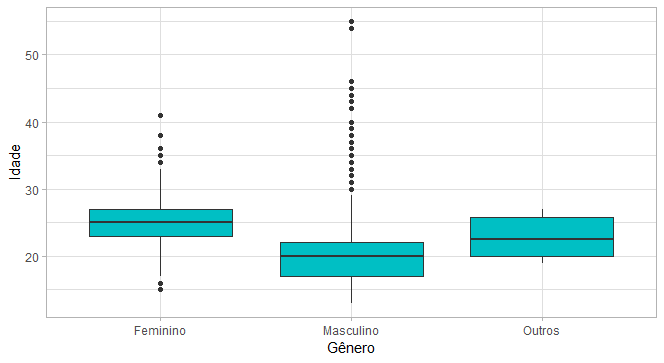
\includegraphics[width=0.45\textwidth]{idadegenero.png}
}
\subfigure[Grafico de pizza com as idades categoricas]{ \label{subfig:grafico2}
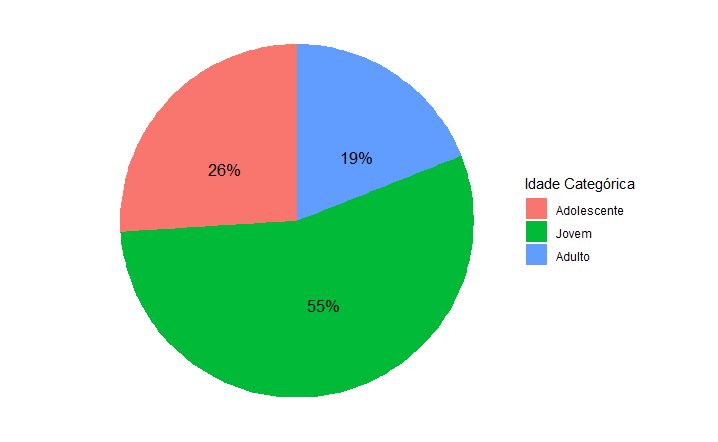
\includegraphics[width=0.45\textwidth]{idadecat.png}
}
\\
\vspace{1cm}
\subfigure[Gênero por horas semanasi jogas]{ \label{subfig:grafico3}
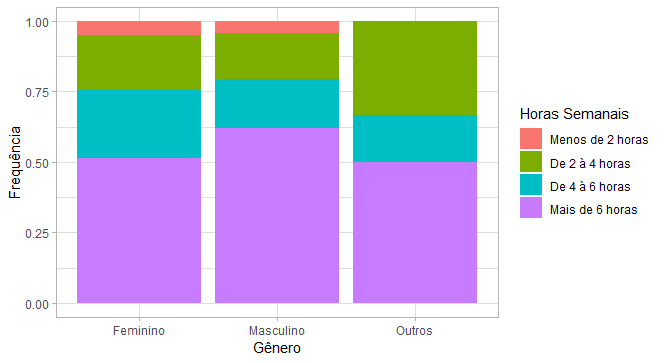
\includegraphics[width=0.45\textwidth]{generohoras.png}
}
\subfigure[Idade categorica por 'Voce acha preço justo?']{ \label{subfig:grafico4}
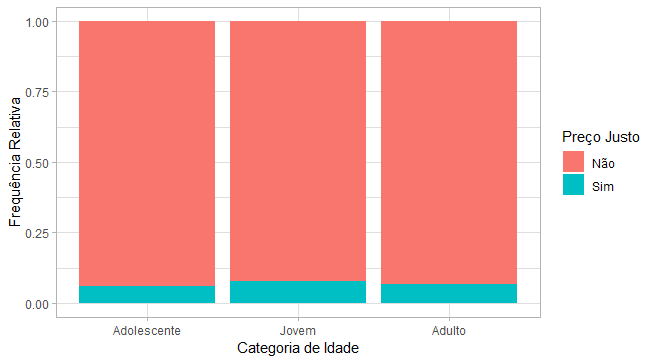
\includegraphics[width=0.45\textwidth]{IdadeJusto.png}
}
\\
\vspace{1cm}
\subfigure[Idade categorica por 'Voce gastou mais do que devia?']{ \label{subfig:grafico5}
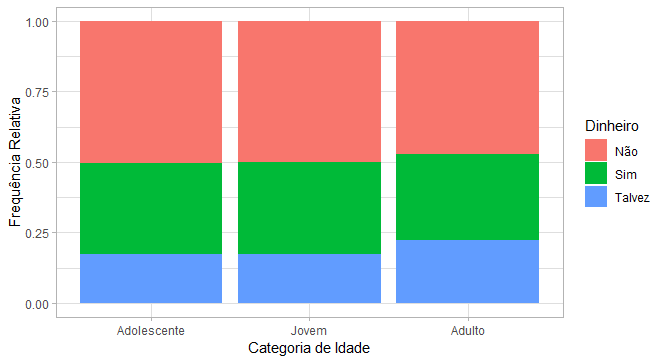
\includegraphics[width=0.45\textwidth]{IdadeDinheiro.png}
}
\subfigure[Tipo de midia por 'Voce gastou mais do que devia?']{ \label{subfig:grafico6}
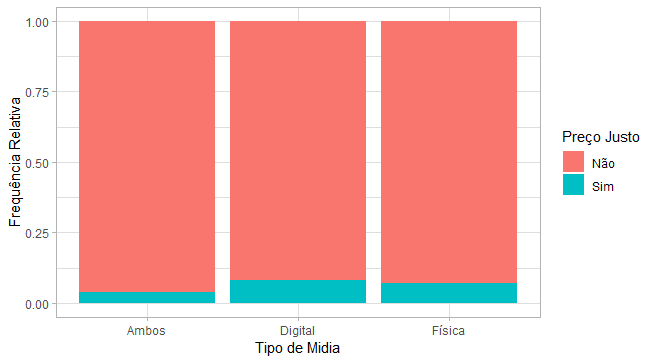
\includegraphics[width=0.4\textwidth]{Midiajusto.png}
}
\end{figure} 

\begin{figure}[H]
\centering

\subfigure[Quantidades de plataformas por quantidade de genero]{ \label{subfig:grafico7}
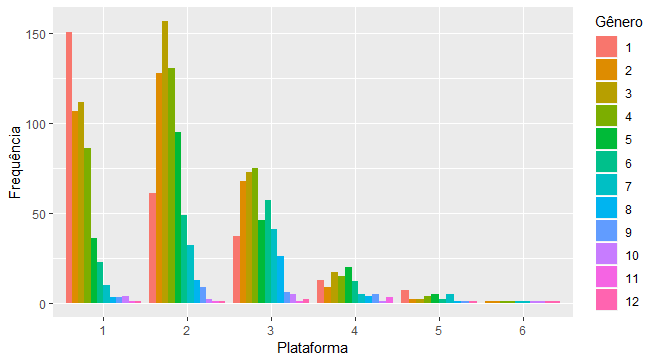
\includegraphics[width=0.7\textwidth]{platxgenero2.png}
}
\\
\vspace{1.5cm}
\subfigure['Você já deixou de jogar por causa dos requisitos mínimos?' ]{ \label{subfig:grafico11}
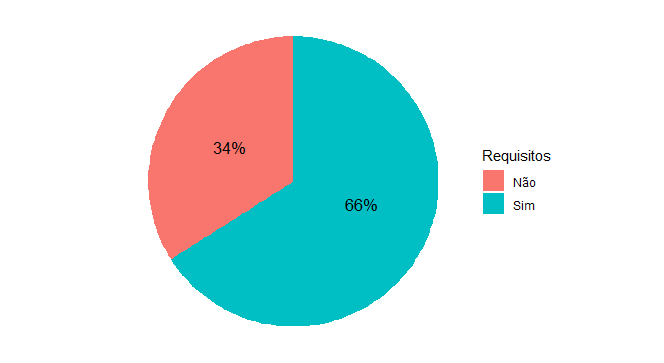
\includegraphics[width=0.45\textwidth]{pizzarequisitos.png}
}
\subfigure[Tipo de Midia]{ \label{subfig:grafico9}
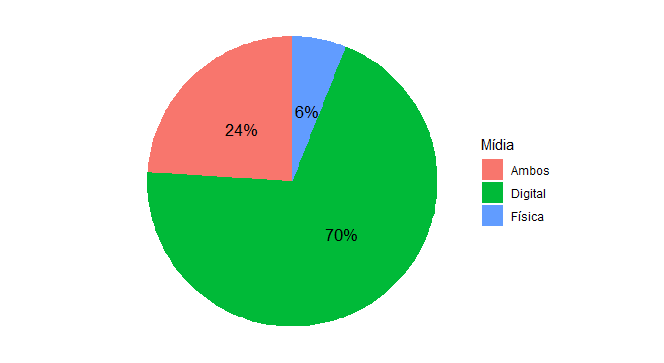
\includegraphics[width=0.45\textwidth]{pizzamidia.png}
}
\\
\vspace{1.5cm}
\subfigure['Você acha justo o preço pago pelos jogos no Brasil?']{ \label{subfig:grafico10}
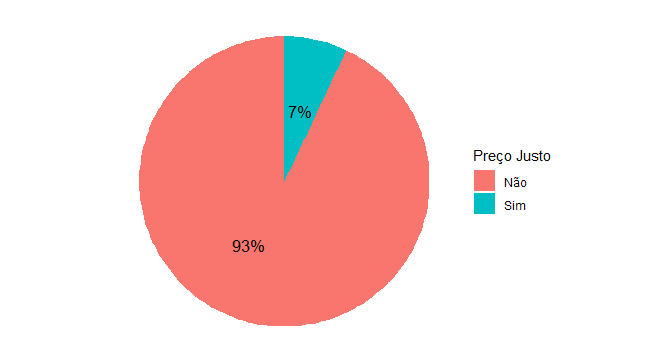
\includegraphics[width=0.45\textwidth]{pizzapreco.png}
}
\subfigure['Já gastou mais dinheiro do que tinha ou devia com jogos?']{ \label{subfig:grafico11}
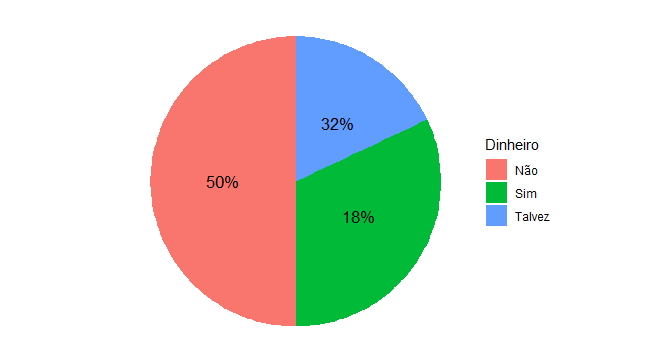
\includegraphics[width=0.45\textwidth]{pizzadinheiro.png}
}
\end{figure}

\begin{figure}[H]
\centering
\subfigure[Grau de escolaridade]{ \label{subfig:grafico12}
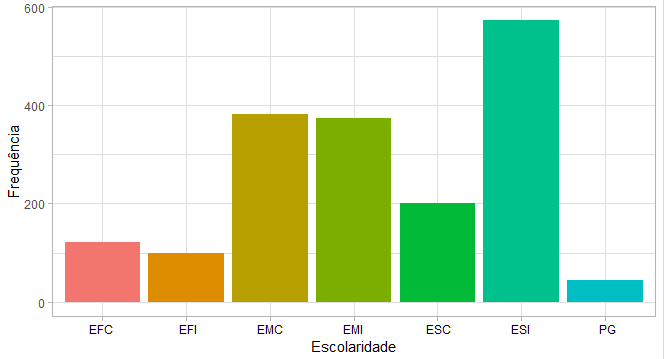
\includegraphics[width=0.6\textwidth]{barescoll.png}
}
\end{figure} 

\noindent
Legenda do grafico \ref{subfig:grafico12}\\
EFC = Ensino Fundamental Completo, EFI = Ensino Fundamental Incompleto, \\EMC = Ensino Médio Completo,
EMI = Ensino Médio Incompleta, ESC = Ensino Superior Completo,\\
ESI = Ensino Superior Incompleto, PG = Pós-Graduação.

\vspace{1cm}


\begin{figure}[H]
\centering
\subfigure[Mapas dos estados com a quantidades de repostas]{ \label{subfig:grafico13}
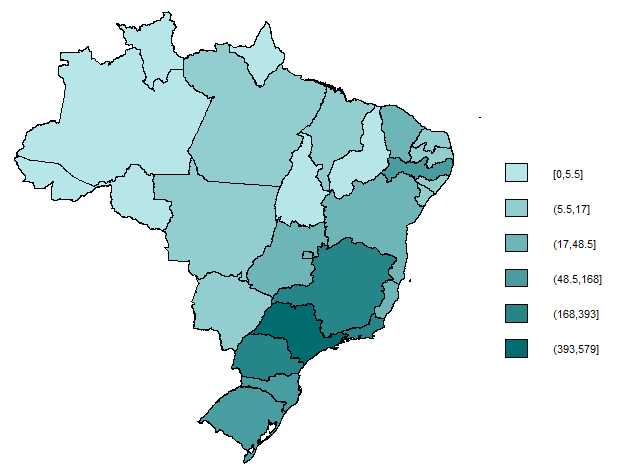
\includegraphics[width=0.7\textwidth]{mapa1.png}
}
\end{figure}


\subsection{Glossário}

\begin{enumerate}[label=(\roman*)]
\item \textit{Downloadeable Content} (DLC) = Expansão de jogos, como: mapas, armas, missões extras, etc ;
\item \textit{Free to Play} (F2P) = Jogos gratuitos ;
\item \textit{Role Playing Game} (RPG) = Jogos de interpretação de personagens, como: Dungeons and Dragons, The Witcher, etc ;
\item \textit{First Person Shooter} (FPS) = Jogos de tiro em primeira pessoa, como: Counter - Strike, Overwatch, Call of Duty, etc ;
\item \textit{Third Person Shooter} (TPS) = Jogos de tiro em terceira pessoa, como: Fortnite, PLAYERUNKNOW`S BATTLEGROUND, Gears of War, etc ;
\item \textit{Multiplayer Online Battle Arena} (MOBA) = Jogos baseados em arena de combate, geralmente entre times, como: DOTA 2, League of Legends, Heroes of the Storm, Heroes of Newerth, etc ;
\item \textit{Massive Multiplayer Online Role Playing Game} (MMORPG) = Jogos de interpretação de personagem online com vários outros jogadores, como: World of Warcraft, Black Desert, TERA, Ragnarok, etc ;
\item \textit{Real Time Strategy} (RTS) = Jogos de estratégia em tempo real, como: Starcraft, Age of Empires, etc;
\item \textit{Puzzle} = Jogos de quebra - cabeça, como: Portal , etc;
\end{enumerate}

\subsection{Formulário}

\begin{question}
	Qual é seu gênero?
	\begin{tasks}(3)
		\task Masculino
		\task Feminino
		\task Outros
	\end{tasks}
\end{question}

\begin{question}
	Qual é seu estado civil?
	\begin{tasks}(3)
	\task Solteiro(a)
	\task Casado(a) ou União Estável
	\task Divorciado(a)
	\task Viúvo(a)
	\task Outro
	\end{tasks}
\end{question}

\begin{question}
 	Qual é sua escolaridade?
	\begin{tasks}(3)
	\task Ensino Fundamental - Incompleto
	
	\task Ensino Fundamental - Completo
	\task Ensino Médio - Incompleto
	\task Ensino Médio - Completo
	
	\task Ensino Superior - Incompleto
	
	\task Ensino Superior - Completo
	
	\task Pós - Graduação
	\end{tasks}
\end{question}
\begin{question}
 	Quais gêneros de jogos você joga atualmente?
	\begin{tasks}(5)
	\task FPS
	\task RPG
	\task RTS
	\task MMORPG
	\task MOBA
	\task Battle Royale
	\task Simuladores
	\task Esportes
	\task Luta
	\task Ação e Aventura
	\task Puzzle
	\task Outros
	\end{tasks}
\end{question}
\begin{question}
	Quantas horas por semana você costuma jogar?
	\begin{tasks}(3)
	\task menos de 2 horas
	\task de 2 à 4 horas
	\task de 4 à 6 horas
	\task mais de 6 horas
	\end{tasks}
\end{question}
\begin{question}
	Quais plataformas você possui na sua casa?
	\begin{tasks}(3)
	\task PC (Steam, Origin, Uplay, etc)
	\task Xbox 360 / Xbox One / Xbox One X / Xbox One S
	\task PS3 / PS4 / PS4 Pro
	\task Wii / Wii U / Switch
	\task Celular e Portáteis
	\task Outros
	\end{tasks}
\end{question}
\begin{question}
	Você tem o hábito de comprar jogos durante a pré-venda?
	\begin{tasks}(3)
	\task Sim
	\task Não
	\end{tasks}
\end{question}
\begin{question}
	Você acha justo o preço pago pelos jogos no Brasil?
	\begin{tasks}(3)
	\task Sim
	\task Não
	\end{tasks}
\end{question}
\begin{question}
	Em que tipo de mídia você consome? (compra, presente ou free to play).
	\begin{tasks}(3)
	\task Fisica
	\task Digital
	\end{tasks}
\end{question}
\begin{question}
	Quais desses produtos relacionados a jogos você costuma comprar?
	\begin{tasks}(3)
	\task DLC / Season Pass
	\task Skins
	\task Aprimoramentos (XP Boost, Gold Boost, etc...)
	\task Merchandising (Camisas, Pelúcias, Action Figures, etc...)
	\task Nenhum
	\task Outros
	\end{tasks}
\end{question}
\begin{question}
 Já foi em alguma conferência ou evento relacionadas aos jogos?
	\begin{tasks}(3)
	\task Sim
	\task Não
	\end{tasks}
\end{question}

\begin{question}
	Já gastou mais dinheiro do que tinha ou devia com jogos?
	\begin{tasks}(3)
	\task Sim
	\task Não 
	\task Talvez
	\end{tasks}
\end{question}

\begin{question}
	Você já deixou de jogar por causa dos requisitos mínimos?
	\begin{tasks}(3)
	\task Sim
	\task Não
	\end{tasks}
\end{question}

\begin{question}
\begin{center}
  \begin{tabular}{| c | c | c | c | }
    \hline
    & Alta Importância & Média Importância & Baixa Importância\\ 
    \hline
    \hline
    Jogabilidade & & & \\ \hline
	Gráficos  & & &\\
    \hline
    Multiplayer & & & \\
    \hline
    Multiplayer Competitivo & & & \\
    \hline
    \makecell{	Tempo de Jogo (Tempo \\ necessário para terminar o jogo)}  & & &\\
    \hline
    Grau de Divertimento & & & \\
    \hline
  \end{tabular}
\end{center}
\end{question}
\textcolor{red}{\underline{OBS}: Nas questões 4, 6, 9, 10 e 13 o voluntario poderia marcar mais de uma opção}

\begin{thebibliography}{9}

\bibitem{R}
R Core Team (2018) R: A Language and Environment for Statistical Computing. R Foundation for Statistical
Computing, Vienna, Austria. \url{http://www.R-project.org/}.

\bibitem{dplyr} 
 Hadley Wickham, Romain François,  Lionel Henry e Kirill Müller (2018) dplyr: A Grammar of Data Manipulation. R package version 0.7.8 \url{https://CRAN.R-project.org/package=dplyr}

\bibitem{R}
R Core Team (2013) R: A Language and Environment for Statistical Computing. R Foundation for Statistical
Computing, Vienna, Austria. \url{http://www.R-project.org/}.

\bibitem{likert}
likert: Analysis and Visualization Likert Items (2016) Jason Bryer and Kimberly Speerschneider, R package version 1.3.5, \url{https://CRAN.R-project.org/package=likert}

\bibitem{stringr}
stringr: Simple, Consistent Wrappers for Common String Operations (2018) Hadley Wickham,
R package version 1.3.1,  \url{https://CRAN.R-project.org/package=stringr}

\bibitem{rgdal}
rgdal: Bindings for the 'Geospatial' Data Abstraction Library (2018) Roger Bivand and Tim Keitt and Barry Rowlingson, R package version 1.3-6, \url{https://CRAN.R-project.org/package=rgdal}
\end{thebibliography}

\end{document}
